% Panel: Sliding Puzzle eta vs H(C) scatter with iso-I_cd contours

% Sliding puzzle agent colors (Okabe-Ito colorblind-safe palette)
\definecolor{spnarrow}{RGB}{204,121,167}
\definecolor{speasy}{RGB}{230,159,0}
\definecolor{sphard}{RGB}{86,180,233}
\definecolor{spwide}{RGB}{0,158,115}
\definecolor{spfull}{RGB}{213,94,0}
\definecolor{sprandom}{RGB}{0,114,178}

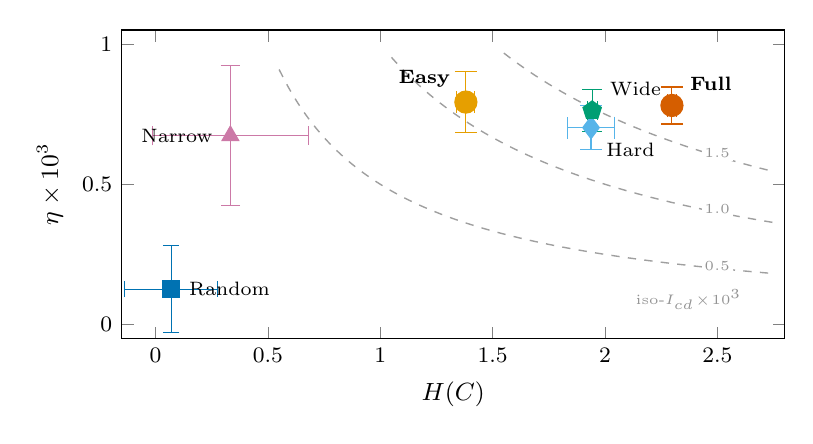
\begin{tikzpicture}
\begin{axis}[
    width=10cm,
    height=5.5cm,
    xlabel={$H(C)$},
    ylabel={$\eta \times 10^3$},
    xlabel style={font=\small},
    ylabel style={font=\small},
    xticklabel style={font=\footnotesize},
    yticklabel style={font=\footnotesize},
    xmin=-0.15, xmax=2.8,
    ymin=-0.05, ymax=1.05,
    every axis plot/.append style={only marks, mark size=3.5pt},
    clip=true,
]

% Iso-I_cd contour lines (hyperbolas: eta = I_cd / H(C))
% I_cd = 0.5 x 10^-3
\addplot[gray!75, line width=0.5pt, dashed, smooth, domain=0.55:2.75, samples=80, no markers]
    {0.5 / x};
% I_cd = 1.0 x 10^-3
\addplot[gray!75, line width=0.5pt, dashed, smooth, domain=1.05:2.75, samples=80, no markers]
    {1.0 / x};
% I_cd = 1.5 x 10^-3
\addplot[gray!75, line width=0.5pt, dashed, smooth, domain=1.55:2.75, samples=80, no markers]
    {1.5 / x};

% Contour labels placed along the curves inside the plot
\node[font=\tiny, text=gray!85, fill=white, inner sep=1pt] at (axis cs:2.5, 0.21) {$0.5$};
\node[font=\tiny, text=gray!85, fill=white, inner sep=1pt] at (axis cs:2.5, 0.41) {$1.0$};
\node[font=\tiny, text=gray!85, fill=white, inner sep=1pt] at (axis cs:2.5, 0.61) {$1.5$};

% Agent points with +/- 1 std error bars in both axes
% Random: eta=0.126+/-0.155, H(C)=0.069+/-0.208
\addplot[color=sprandom, mark=square*, mark size=3pt,
    error bars/.cd, x dir=both, x explicit, y dir=both, y explicit]
    coordinates {(0.069, 0.126) +- (0.208, 0.155)};
\node[font=\scriptsize, anchor=west, xshift=3pt] at (axis cs:0.069, 0.126) {Random};

% Narrow: eta=0.673+/-0.249, H(C)=0.333+/-0.346
\addplot[color=spnarrow, mark=triangle*, mark size=3.5pt,
    error bars/.cd, x dir=both, x explicit, y dir=both, y explicit]
    coordinates {(0.333, 0.673) +- (0.346, 0.249)};
\node[font=\scriptsize, anchor=east, xshift=-3pt] at (axis cs:0.333, 0.673) {Narrow};

% Easy: eta=0.793+/-0.110, H(C)=1.381+/-0.040
\addplot[color=speasy, mark=*, mark size=4pt,
    error bars/.cd, x dir=both, x explicit, y dir=both, y explicit]
    coordinates {(1.381, 0.793) +- (0.040, 0.110)};
\node[font=\scriptsize, anchor=south east, xshift=-2pt, yshift=2pt] at (axis cs:1.381, 0.793) {\textbf{Easy}};

% Hard: eta=0.702+/-0.079, H(C)=1.938+/-0.105
\addplot[color=sphard, mark=diamond*, mark size=4pt,
    error bars/.cd, x dir=both, x explicit, y dir=both, y explicit]
    coordinates {(1.938, 0.702) +- (0.105, 0.079)};
\node[font=\scriptsize, anchor=north west, xshift=2pt, yshift=-2pt] at (axis cs:1.938, 0.702) {Hard};

% Wide: eta=0.763+/-0.076, H(C)=1.943+/-0.022
\addplot[color=spwide, mark=pentagon*, mark size=3.5pt,
    error bars/.cd, x dir=both, x explicit, y dir=both, y explicit]
    coordinates {(1.943, 0.763) +- (0.022, 0.076)};
\node[font=\scriptsize, anchor=south west, xshift=3pt, yshift=2pt] at (axis cs:1.943, 0.763) {Wide};

% Full: eta=0.781+/-0.066, H(C)=2.298+/-0.021
\addplot[color=spfull, mark=*, mark size=4pt,
    error bars/.cd, x dir=both, x explicit, y dir=both, y explicit]
    coordinates {(2.298, 0.781) +- (0.021, 0.066)};
\node[font=\scriptsize, anchor=south west, xshift=3pt, yshift=2pt] at (axis cs:2.298, 0.781) {\textbf{Full}};

% Contour annotation at bottom right
\node[font=\tiny, text=gray!85, anchor=south east] at (axis cs:2.65, 0.02) {iso-$I_{cd} \!\times\! 10^3$};

\end{axis}
\end{tikzpicture}
